\pdfoutput=1
% main.tex -- arXiv submission source.
% Build: pdflatex main && bibtex main && pdflatex main && pdflatex main
% (or: latexmk -pdf main). Submit main.tex, main.bbl and figures/*.png.
\documentclass[11pt]{article}

\usepackage[T1]{fontenc}
\usepackage[utf8]{inputenc}
\usepackage{lmodern}
\usepackage[a4paper,margin=1in]{geometry}
\usepackage{amsmath,amssymb,amsthm}
\usepackage{booktabs}
\usepackage{tabularx}
\usepackage{graphicx}
\usepackage{xcolor}
\usepackage{listings}
\usepackage{enumitem}
\usepackage[round,authoryear]{natbib}
\usepackage[colorlinks=true,linkcolor=blue!50!black,citecolor=blue!50!black,urlcolor=blue!50!black]{hyperref}

\graphicspath{{figures/}}

% ---------------------------------------------------------------- macros
\newcommand{\code}[1]{\texttt{\detokenize{#1}}}
\newcommand{\pf}[1]{\textit{#1}}
\newcommand{\stipmark}{\texttt{\#~STIPULATION}}
\newcommand{\Def}[1]{D#1}
\newcommand{\Thm}[1]{T#1}
\newcommand{\LA}{\mathrm{LA}}
\newcommand{\Merge}{\mathrm{Merge}}
\newcommand{\Select}{\mathrm{Select}}
\newcommand{\Triggers}{\mathrm{Triggers}}
\newcommand{\Label}{\mathrm{Label}}
\newcommand{\TPF}{\mathrm{TransferPF}}
\newcommand{\TLF}{\mathrm{TransferLF}}
\newcommand{\CT}{\mathrm{Cyclic\text{-}Transfer}}
\newcommand{\pair}[1]{\langle #1 \rangle}

\theoremstyle{definition}
\newtheorem{definition}{Definition}
\theoremstyle{plain}
\newtheorem{observation}{Observation}

\lstset{
  basicstyle=\ttfamily\small,
  keywordstyle=\color{black!75}\bfseries,
  commentstyle=\itshape\color{black!55},
  columns=fullflexible,
  frame=leftline,
  framesep=6pt,
  xleftmargin=12pt,
  breaklines=true,
  language=Python,
  showstringspaces=false,
}

\title{An executable Collins \& Stabler (2016):\\[2pt]
\large a self-validating implementation of a formalization of minimalist syntax}

% TODO: replace with the author's name and affiliation before submission.
\author{Author Name\\
  \texttt{norbmor@gmail.com}}

\date{}

\begin{document}
\maketitle

% ---------------------------------------------------------------- abstract
\begin{abstract}
\citet{CollinsStabler2016} give an axiomatization of minimalist syntax:
forty-four definitions, five Chain-based variants and fourteen theorems,
precise enough to decide whether a given sequence of operations is a
derivation. We transcribe the axiomatization into Python,
one named function per definition and theorem, and wrap it in a driver that
refuses any step the definitions do not license; a derivation object can
therefore only contain licensed steps. Seventeen derivations, eight from
the paper and nine added, validate against the definition of a derivation
and against Theorems 5--10, and 76 automated checks pass. The implementation
reproduces the paper's argument against the ``plug-back-in'' model of
Transfer: remnant movement inside one phase is spelled out correctly, but the
paper's two-phase example (21) is pronounced \pf{how likely John to win you
think that John is}, and that derivation still converges. An implementation
of the paper's Section~12 alternative pronounces it correctly. We also report
three results the paper does not state. Theorem~4, the correspondence between
token-based and Chain-based objects, fails on exhaustively enumerated
fragments from three Merge nodes on, under every reading of its misprinted
locality condition. The Section~12 sketch works under one reading of ``$W$
minus those already transferred'' and makes successive-cyclic movement
underivable under the other. And with the unordered trigger features the
paper assumes, adding selection to Triggered Merge still admits the
$[_{\mathrm{TP}}\ \mathrm{vP}\ [_{\mathrm{T'}}\ \mathrm{T}\ \mathrm{DP}]]$
orders the paper leaves to other constraints.
\end{abstract}

\medskip
\noindent\textbf{Keywords:} minimalist syntax; formalization; Merge;
phases; Transfer; remnant movement; executable specification

% ================================================================ 1
\section{Introduction}
\label{sec:intro}

Formal treatments of minimalist syntax usually take one of two routes. One
abstracts away from the details of the theory to obtain a grammar formalism
with well-understood computational properties, as Minimalist Grammars do
\citep{Stabler1997,Stabler2011}. The other stays close to the theory as
syntacticians state it and makes its notions precise.
\citet{CollinsStabler2016} (henceforth C\&S) take the second route. They
define lexical items, workspaces, Select, Merge, occurrences, derivations,
labels, Transfer and convergence, and they state theorems about them,
including the Phase Impenetrability Condition (PIC), the No-Tampering
Condition (NTC) and the Extension Condition.

The definitions are explicit enough to be run as a program, and this report
describes what happens when they are. We implemented them as written and
checked whether the paper's derivations go through and whether its theorems
hold. Where the prose says more than the definitions, we recorded the choice
we had to make.

Section~\ref{sec:impl} describes the implementation: about 1{,}600 lines of
standard-library Python covering \Def{1}--\Def{44}, the Chain-based variants
\Def{7}$'$ and \Def{13}$'$--\Def{16}$'$, and \Thm{1}--\Thm{14}. Each definition
and theorem has a function or class tagged with its number. The core is a
derivation driver that checks every step against \Def{14}/\Def{38} and
raises an error naming the definition an illegal step violates
(Section~\ref{sec:driver}). Section~\ref{sec:validation} lists the
derivations it validates. Section~\ref{sec:remnant} confirms the paper's
argument that the plug-back-in model of Transfer mishandles remnant movement
across phases, and shows that the faulty derivation converges.
Section~\ref{sec:ntc} implements the NTC-respecting alternative of the
paper's Section~12 and identifies two points the sketch leaves open: which
parts of the workspace become inaccessible, and what a stage is.
Section~\ref{sec:t4} checks Theorem~4 exhaustively on bounded fragments,
where it fails. Section~\ref{sec:selection} enumerates all derivations from
one lexical array under Triggered Merge with and without selection, and finds
the word orders that the paper raises as a problem and leaves open.

Definition and theorem numbers follow the 2016 journal version throughout. We
write \Def{n} for Definition~n and \Thm{n} for Theorem~n of C\&S. The
implementation was first written against the December 2011 manuscript
\citep{CollinsStabler2011}, which numbers things differently and contains
definitions the published version dropped; Appendix~\ref{app:2011} records
what changed.

% ================================================================ 2
\section{The axiomatization}
\label{sec:background}

This section summarizes the parts of C\&S that the results depend on. We
paraphrase closely and keep C\&S's numbering.

\subsection{Lexical items, stages and derivations}

A lexical item is a triple $\pair{\mathrm{Sem},\mathrm{Syn},\mathrm{Phon}}$
(\Def{2}); a lexical item token is a pair $\pair{\mathrm{LI},k}$ with an
index $k$ (\Def{5}); a lexical array is a finite set of tokens (\Def{6}). A
syntactic object is a token or a set of syntactic objects (\Def{7}).

\begin{definition}[Stage, Select, Merge; \Def{10}, \Def{12}, \Def{13}]
A \emph{stage} is a pair $S = \pair{\LA, W}$ of a lexical array and a set of
syntactic objects, the \emph{workspace}. If $A \in \LA$ then
$\Select(A,S) = \pair{\LA - \{A\},\ W \cup \{A\}}$. For distinct syntactic
objects $A,B$, $\Merge(A,B) = \{A,B\}$.
\end{definition}

\begin{definition}[Derivation; \Def{14}]
A derivation from lexicon $L$ is a finite sequence of stages
$\pair{S_1,\dots,S_n}$ with $S_i = \pair{\LA_i, W_i}$ such that (i) every
token in $\LA_1$ is a token of an item in $L$; (ii) $W_1 = \{\}$; and (iii)
for all $i<n$, either $S_{i+1} = \Select(A, S_i)$ for some $A\in\LA_i$
(\emph{derive-by-Select}), or $\LA_{i+1} = \LA_i$ and for some $A,B$:
(a) $A \in W_i$, (b) $A$ contains $B$ (internal Merge) or $W_i$ immediately
contains $B$ (external Merge), and (c)
$W_{i+1} = (W_i - \{A,B\}) \cup \{\Merge(A,B)\}$ (\emph{derive-by-Merge}).
\end{definition}

\noindent
Requiring an empty final lexical array and a single root is a separate
notion, the object derived (\Def{15}). Occurrences are paths from the root
(\Def{16}--\Def{17}), and sisterhood and c-command are defined on them
(\Def{18}--\Def{22}).

\subsection{Triggers and labels}

Each lexical item carries a set of trigger features (\Def{25}).
$\Triggers$ is any function satisfying three conditions (\Def{26}): a token
returns all its trigger features; a set $\{B,C\}$ with $\Triggers(B)\neq\{\}$
and $\Triggers(C)=\{\}$ returns $\Triggers(B)-\{\mathrm{TF}\}$ for
``a particular one'' $\mathrm{TF}$, ``determined by $B$ and $C$''; otherwise it
is undefined.

\begin{definition}[Triggered Merge; \Def{27}]
For syntactic objects $A,B$ with $\Triggers(A)\neq\{\}$ and
$\Triggers(B)=\{\}$, $\Merge(A,B)=\{A,B\}$.
\end{definition}

\noindent
The label of $\{A,B\}$ is the label of the trigger-bearing member
(\Def{28}); maximal, minimal and intermediate projections, complements and
specifiers are defined from it (\Def{29}--\Def{33}). C\&S state explicitly
that trigger features are \emph{not} ordered, and ask what then prevents
$[_{\mathrm{TP}}\ \mathrm{vP}\ [_{\mathrm{T'}}\ \mathrm{T}\ \mathrm{DP}]]$,
leaving the answer to ``other constraints'' such as the NTC.

\subsection{Transfer}

A strong phase is a maximal projection labelled by Comp or by a transitive or
unergative v (\Def{35}).

\begin{definition}[Cyclic-Transfer; \Def{36}]
For a strong phase $SO$ in a derivable workspace with complement $A$ of its
label, $\CT(SO)$ is obtained from $SO$ by replacing $A$ with
$\pair{\TPF(SO,A),\ \TLF(SO,A)}$.
\end{definition}

\noindent
Because the result must feed further Merge, \Def{37} revises \Def{7} so that
$\CT(SO)$ is a syntactic object, though the inserted pair itself is not. The
definition of a derivation is extended (\Def{38}) with a third clause:
\emph{derive-by-Transfer} applies to a strong phase $SO\in W_i$ that contains
no other strong phase with an untransferred complement, and replaces it either
by $\mathrm{Transfer}(SO,SO)$, which ends the derivation, or by $\CT(SO)$.
C\&S call this the \emph{plug-back-in} model. The PIC follows as \Thm{14},
since Merge is defined only on syntactic objects and the inserted pair does
not contain any.

\begin{definition}[Finality; \Def{40}]
$A \in \{A,B\}$ is \emph{final} in $SO$ iff there is no $C$ contained in (or
equal to) $SO$ such that $A\in C$ and $C$ contains $\{A,B\}$. Otherwise $A$ is
non-final in $SO$.
\end{definition}

\noindent
$\TPF$ (\Def{41}) spells out a token as its Phon; spells out $\{X,Y\}$ as
$\TPF(X)\frown\TPF(Y)$ when both are final and $Y$ is the complement of $X$
or $X$ the specifier of $Y$; skips a non-final member; and spells out an
inserted pair $\pair{\mathrm{PHON},\mathrm{SEM}}$ as PHON. Clause (b) makes
specifier--head--complement order universal \citep{Kayne1994}. $\TLF$
(\Def{39}) keeps the Sem and index of every token and the set structure. A
derivation converges at CI iff the final SEM is interpretable, at SM iff the
final PHON is, and converges iff both hold (\Def{42}--\Def{44}).

\subsection{The Chain-based digression and Theorem 4}

Section~5 of C\&S defines a system without indices, in which a syntactic
object is a pair $\pair{S,P}$ of a structure and a path (\Def{7}$'$,
\Def{16}$'$). Internal Merge records the path to the moved item, subject to a
locality condition \Def{14}$'$(c). Theorem~4 asserts a one-to-one, onto,
structure-preserving correspondence between token-based objects up to
renumbering, $[T(\mathrm{Lex})]$ (excluding merges of renumberings), and
Chain-based objects $C(\mathrm{Lex})$. The proof is in an appendix that was
not published.

% ================================================================ 3
\section{Implementation}
\label{sec:impl}

\subsection{Design}

The code follows the paper as closely as we could make it. Every definition
and theorem has a counterpart tagged with its number, so the two can be read
side by side (Table~\ref{tab:map}). The code enforces only what the paper
states: \code{triggered_merge}, for instance, has no category-matching check,
because \Def{27} checks only that one argument has triggers and the other has
none. Where the paper leaves a choice open, the code makes one and marks it
\stipmark{} (Table~\ref{tab:stip}).

Lexical items are immutable value objects, and tokens pair an item with an
index. Complex syntactic objects are Python \code{frozenset}s, which gives set
identity and extensionality directly; an internally merged object is simply
a member of two sets. Occurrences are tuples of objects forming a path from the root
(\Def{16}). The inserted Transfer pair is a separate type which the
predicate \code{is_syntactic_object} accepts only as a member of a
Cyclic-Transfer output, as \Def{37} requires.

\begin{table}[t]
\centering
\small
\begin{tabularx}{\linewidth}{@{}lX@{}}
\toprule
Section of C\&S & Counterparts in \code{cs2016.py} \\
\midrule
\S2 Preliminaries & \code{UniversalGrammar} (\Def{1}), \code{LexicalItem} (\Def{2}), \code{Lexicon} (\Def{3}), \code{LIToken} (\Def{5}), \code{lexical_array} (\Def{6}), \code{is_syntactic_object} (\Def{7}/\Def{37}), \code{contains} (\Def{9}) \\
\S3 Workspaces & \code{Stage} (\Def{10}), \code{select} (\Def{12}), \code{merge} (\Def{13}), \code{is_derivation} (\Def{14}), \code{derived_object} (\Def{15}) \\
\S4 Occurrences & \code{positions} (\Def{16}--\Def{17}), \code{are_sisters} (\Def{19}), \code{occ_c_commands} (\Def{22}), \code{theorem1_holds}--\code{theorem3_holds} \\
\S5 Chains & \code{ChainSO} (\Def{7}$'$), \code{chain_merge} (\Def{13}$'$), \code{is_chain_derivation} (\Def{14}$'$), \code{theorem4_report} (\Thm{4}) \\
\S6 Properties & \code{is_binary_branching} (\Def{24}, \Thm{5}), \code{satisfies_ntc} (\Thm{8}), \code{satisfies_extension} (\Thm{9}), \code{satisfies_inclusiveness} (\Thm{10}) \\
\S7 Labels & \code{triggers} (\Def{26}), \code{triggered_merge} (\Def{27}), \code{label} (\Def{28}), \code{complement_of} (\Def{32}), \code{specifier_of} (\Def{33}) \\
\S8 Transfer & \code{is_strong_phase} (\Def{35}), \code{cyclic_transfer} (\Def{36}), \code{derives_by_transfer} (\Def{38}), \code{pic_blocks} (\Thm{14}) \\
\S9--10 Interfaces & \code{transfer_lf} (\Def{39}), \code{is_final} (\Def{40}), \code{transfer_pf} (\Def{41}) \\
\S12 Alternative & \code{NTCStage}, \code{is_accessible}, \code{cyclic_transfer_ntc}, \code{NTCDerivation} \\
\S13 Convergence & \code{converges_at_ci} (\Def{42}), \code{converges_at_sm} (\Def{43}), \code{converges} (\Def{44}) \\
\bottomrule
\end{tabularx}
\caption{Excerpt of the definition map. The full map, covering all 115
top-level functions and classes, is in the repository README.}
\label{tab:map}
\end{table}

\subsection{Stipulations}

Table~\ref{tab:stip} lists every point at which the implementation had to
choose. Stipulation~1 is inert under \Def{27} (Section~\ref{sec:selection});
stipulation~5 is not (Section~\ref{sec:ntc}).

\begin{table}[t]
\centering
\small
\begin{tabularx}{\linewidth}{@{}rlX@{}}
\toprule
\# & Where & Choice made \\
\midrule
1 & \Def{26}(ii) & Which trigger feature is checked: the paper says only ``a particular one, determined by $B$ and $C$''. The default checks the lowest-ranked one. \\
2 & \Def{38} & The Transfer clause says nothing about $\LA_{i+1}$. We require $\LA_{i+1}=\LA_i$, as in derive-by-Merge. \\
3 & \Def{36} & ``Replacing $A$'' is read positionally: the complement occurrence is replaced. \\
4 & \Def{14}$'$(c) & Read literally, the locality condition blocks every internal Merge, the paper's own (7$'$) included. We read it as ``the path does not pass a higher occurrence of $B$''. \\
5 & \S12 & ``$W$ minus those already transferred'' is read per occurrence by default; the per-object reading is selectable. \\
6 & display & \code{LexicalItem.name} and \code{.cat} exist only for printing. \\
\bottomrule
\end{tabularx}
\caption{Stipulations. Each is marked \stipmark{} in the source.}
\label{tab:stip}
\end{table}

\subsection{The self-validating driver}
\label{sec:driver}

The \code{Derivation} class holds a sequence of stages. Each method constructs
the next stage and, before accepting it, asserts that the previous stage
derives it by one of the clauses of \Def{14}/\Def{38}. A derivation object
therefore cannot contain an unlicensed step. The following derives C\&S's
example (18), \pf{John fell}, with \pf{John} raising from the complement of
unaccusative \pf{fall} to Spec,TP:

\begin{lstlisting}
from derivations import LEX
from cs2016 import Derivation, labelled_bracket

d = Derivation(LEX, [LEX.token("fall", 1), LEX.token("John", 2),
                     LEX.token("T_V", 3), LEX.token("Comp", 4)])
d.select("fall", 1).select("John", 2).merge_roots()
d.select_and_merge("T_V", 3)
d.internal_merge(LEX.token("John", 2))
d.select_and_merge("Comp", 4)
print(labelled_bracket(d.root))
# [CP Comp4 [TP John2 [T' T_V3 [VP fall1 <John2>]]]]
d.transfer()      # D38(a): Transfer(CP, CP)
d.check()
\end{lstlisting}

\noindent
Illegal moves raise with the number of the definition they violate:
selecting a token outside the lexical array reports \Def{12}; merging a
trigger-less selector reports \Def{27}; transferring a phase that contains a
phase with an untransferred complement reports \Def{38}. A second driver,
\code{NTCDerivation}, implements the Section~12 alternative
(Section~\ref{sec:ntc}).

\subsection{Extensions}

\code{extensions.py} adds two things that are not in C\&S, kept separate from
the transcription: a \emph{selectional} Merge, in which a trigger feature
must match the category of the merged object, with ranked or unranked trigger
features; and an enumerator over all complete derivations (\Def{15}) from a
lexical array. Because Select shrinks the lexical array and every Triggered
Merge checks one feature, the state graph from a finite array is finite and
acyclic, so exhaustive enumeration terminates.

% ================================================================ 4
\section{Validation}
\label{sec:validation}

Two test suites run without third-party dependencies:
\code{test_cs2016.py} has 55 checks, one per definition cluster, theorem,
paper example or finding; \code{test_sentences.py} has 21 checks over added
constructions plus a smoke test that draws every derivation. All 76 pass.

Table~\ref{tab:coverage} lists the seventeen derivations the driver
validates. Every one satisfies \Def{14}/\Def{38} and \Def{15}, and Theorems
\Thm{5} (binary branching), \Thm{6} (unique root occurrences), \Thm{7}
(two occurrences iff internal Merge), \Thm{8} (NTC) at Select and Merge,
\Thm{9} (Extension) and \Thm{10} (Inclusiveness). Theorems \Thm{1}--\Thm{3}
are checked on every object built. PF and convergence are computed by
\Def{41}--\Def{44}.

\begin{table}[t]
\centering
\footnotesize
\setlength{\tabcolsep}{3.5pt}
\begin{tabular}{@{}llrrlcc@{}}
\toprule
Derivation & Source & Steps & C-T & PF & CI & SM \\
\midrule
\code{external_merge_6}             & (6)/(8)    &  5 & 0 & ---  & --- & --- \\
\code{internal_merge_7}             & (7)        &  4 & 0 & ---  & --- & --- \\
\code{two_trigger_features_15}      & (15)       &  4 & 0 & ---  & --- & --- \\
\code{vp_see_chris}                 & (16)/(17)  &  3 & 0 & ---  & --- & --- \\
\code{john_fell}                    & (18)       &  9 & 0 & \pf{John fell} & yes & yes \\
\code{remnant_movement}             & (19)/(20)  & 16 & 0 & \pf{how likely to win John is} & yes & yes \\
\code{remnant_across_phases}        & (21)       & 31 & 2 & \pf{how likely John to win \dots\ John is} & yes & yes \\
\code{crashing}                     & \Def{42}   & 14 & 1 & \pf{John see Chris} & no & yes \\
\midrule
\code{john_sees_chris}              & added      & 14 & 1 & \pf{John see Chris} & yes & yes \\
\code{successive_cyclic_wh}         & added      & 31 & 3 & \pf{who you think John will see} & yes & yes \\
\code{john_seems_to_win}            & added      & 13 & 0 & \pf{John seem to win} & yes & yes \\
\code{you_wonder_who_john_will_see} & added      & 29 & 3 & \pf{you wonder who John will see} & yes & yes \\
\code{john_gives_mary_flowers}      & added      & 16 & 1 & \pf{John Mary give flowers} & yes & yes \\
\code{mary_praises_john}            & added      & 14 & 1 & \pf{Mary praise John} & yes & yes \\
\code{mary_not_praise_john}         & added      & 16 & 1 & \pf{Mary not praise John} & yes & yes \\
\code{sue_thinks_john_fell}         & added      & 22 & 2 & \pf{Sue think John fell} & yes & yes \\
\code{who_does_sue_think_fell}      & added      & 25 & 2 & \pf{who Sue think fell} & yes & yes \\
\bottomrule
\end{tabular}
\caption{Derivations validated by the driver. \emph{Steps} counts Select,
Merge and Transfer operations; \emph{C-T} counts Cyclic-Transfer steps. The
first four have no Transfer step, so \Def{42}--\Def{44}, which inspect
$W_n=\{\pair{\mathrm{PHON},\mathrm{SEM}}\}$, do not apply; the first two use
untriggered Merge (\Def{13}), as Section~3 of C\&S does. \code{crashing}
uses a lexical item that is uninterpretable at CI by stipulation.}
\label{tab:coverage}
\end{table}

The PIC (\Thm{14}) and successive cyclicity both follow from the
definitions; neither is coded separately. The PIC follows from a typing fact: Cyclic-Transfer replaces the complement by a
pair that \Def{37} does not count as a syntactic object, and Merge is defined
only on syntactic objects. Successive cyclicity is forced in the same
indirect way. In \code{successive_cyclic_wh}, \pf{who} ends with five
occurrences (in situ, embedded v* edge, embedded Spec,CP, matrix v* edge,
matrix Spec,CP), exactly one of them final. Without the step to the matrix
v* edge, Cyclic-Transfer at that vP buries \pf{who} in the transferred VP and
the final movement is refused (Figure~\ref{fig:wh}).

\begin{figure}[t]
  \centering
  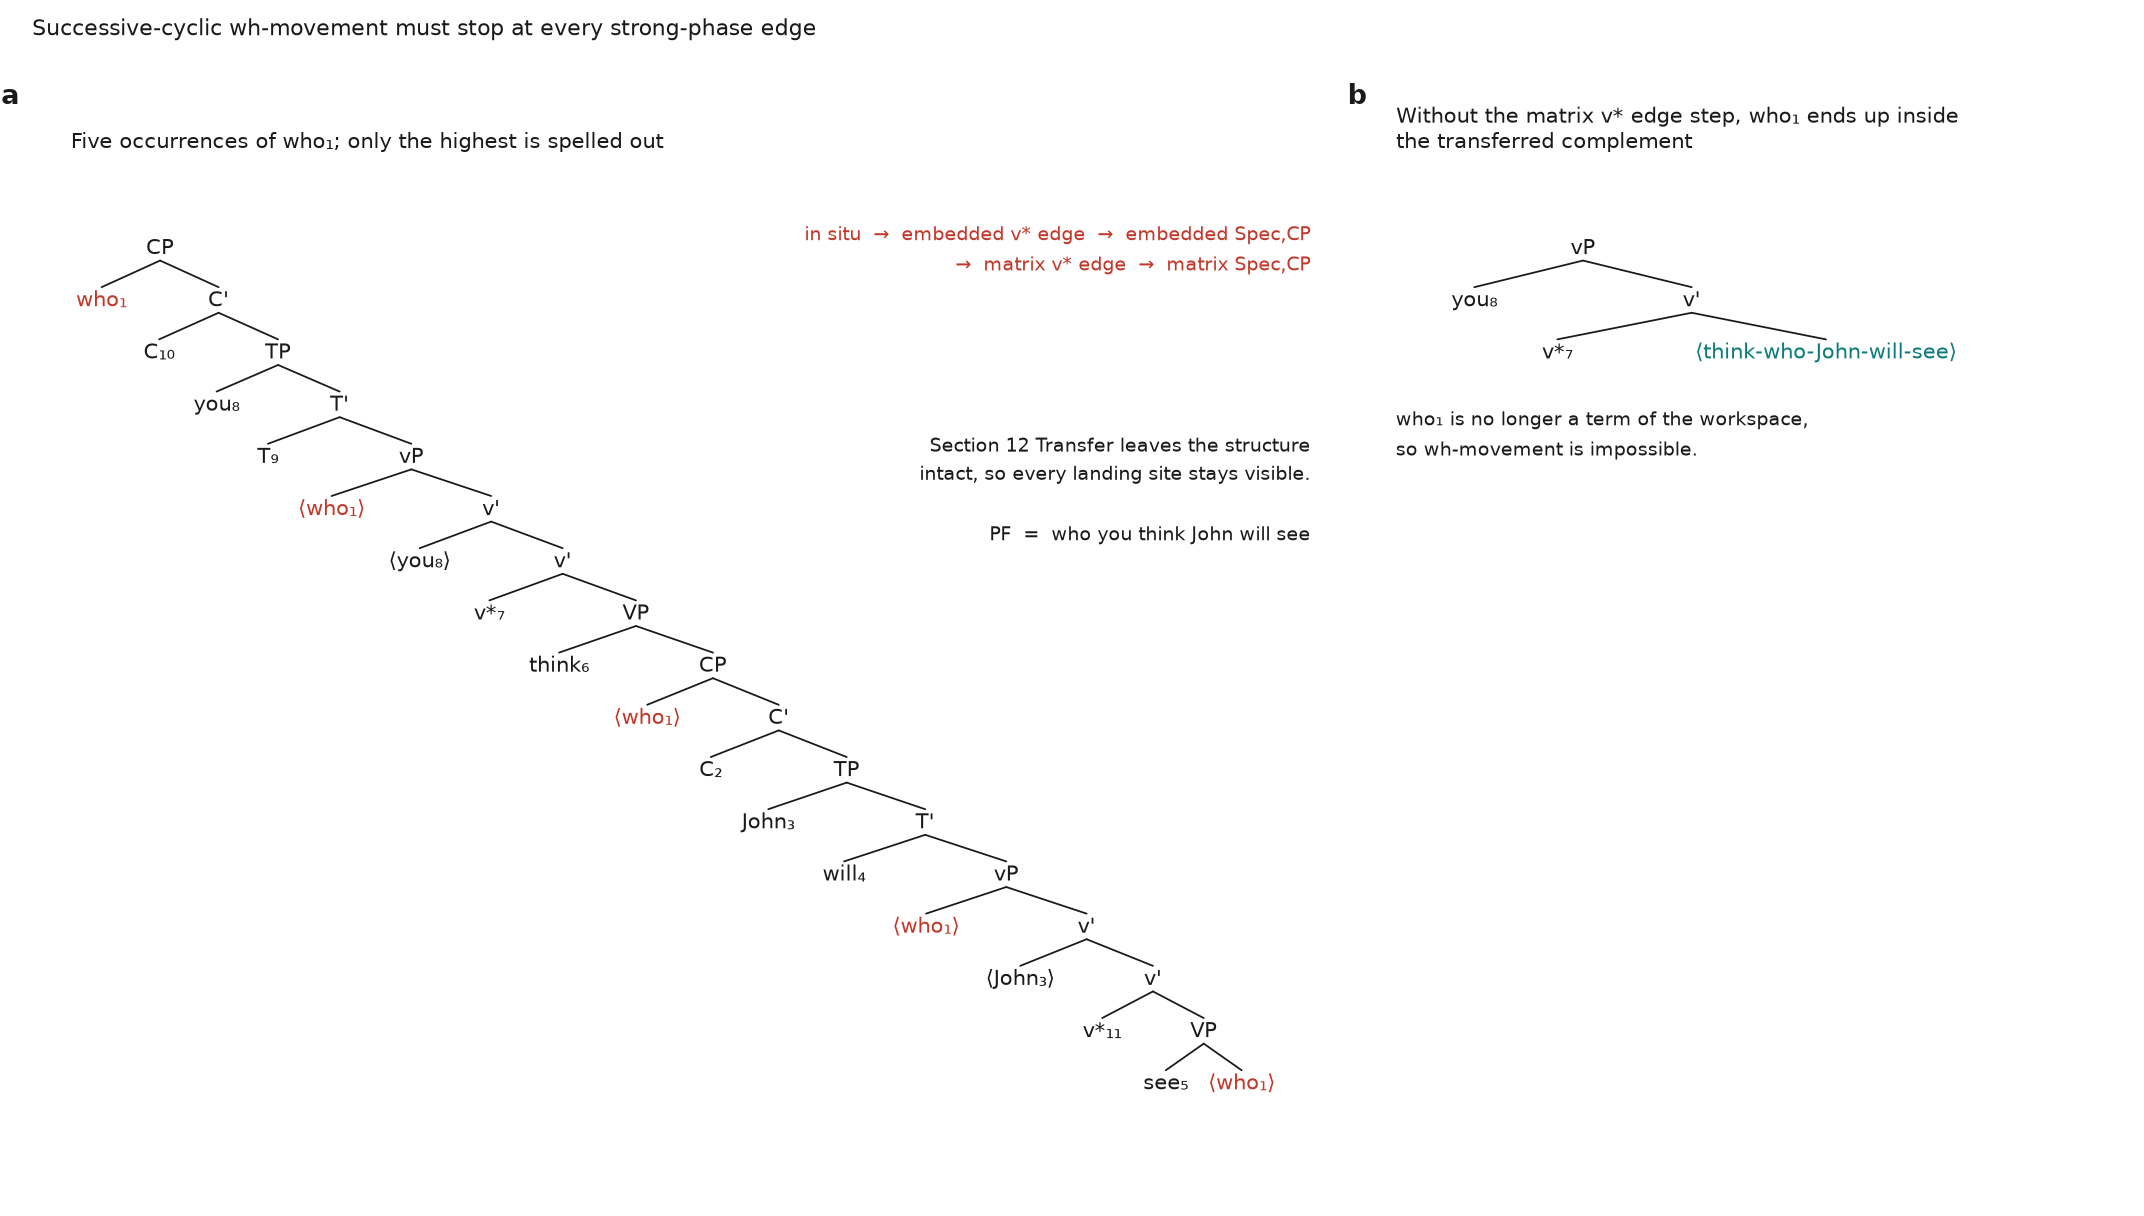
\includegraphics[width=\linewidth]{successive_cyclic_wh.png}
  \caption{Successive cyclicity is forced. \textbf{(a)} The five occurrences
  of \pf{who}$_1$, drawn under the Section~12 Transfer, which leaves the
  workspace intact. \pf{John}$_3$ is merged in the embedded Spec,vP and
  raises to Spec,TP of \pf{will}. \textbf{(b)} Without the step to the
  matrix v* edge, \pf{who}$_1$ is inside the complement transferred at that
  phase, and the final movement is refused (\Thm{14}).}
  \label{fig:wh}
\end{figure}

% ================================================================ 5
\section{Remnant movement and the plug-back-in model}
\label{sec:remnant}

\Def{40} defines finality structurally. In C\&S's (20d), the TP has
\pf{John} as a member and contains $\{\mathit{John},\{\mathit{to},
\mathit{win}\}\}$, so \pf{John} is non-final in \emph{both} copies of the
moved DegP. A single Transfer at (20d) yields \pf{how likely to win John is}
(Figure~\ref{fig:remnant}a). If Transfer applies at (20c) instead, before the
remnant moves, the DegP is inside the transferred TP and cannot move
(\Thm{14}). Both facts are tested.

C\&S argue that this solution does not survive a second phase, and the
driver confirms it. In (21) the embedded TP has been replaced by its interface pair
before the matrix CP is spelled out, so at the matrix level nothing contains
$\{\mathit{John},\{\mathit{to},\mathit{win}\}\}$ while having \pf{John} as a
member. \pf{John} is final again and is pronounced twice
(Figure~\ref{fig:remnant}b):

\begin{quote}
\pf{how likely John to win you think that John is}
\end{quote}

\begin{observation}
\label{obs:converges}
The derivation of (21) under the plug-back-in model is licensed at every step
by \Def{38} and converges at both interfaces (\Def{42}--\Def{44}). The
convergence definitions inspect only features, so they cannot detect a
string that misrepresents the structure.
\end{observation}

\begin{observation}
\label{obs:onephase}
The same failure arises inside a single phase. \Def{38} also licenses
Cyclic-Transfer at (20d) followed by $\mathrm{Transfer}(SO,SO)$. In that
derivation the TP is plugged back in before the final spell-out, and (20)
comes out as \pf{how likely John to win John is}.
\end{observation}

\begin{figure}[t]
  \centering
  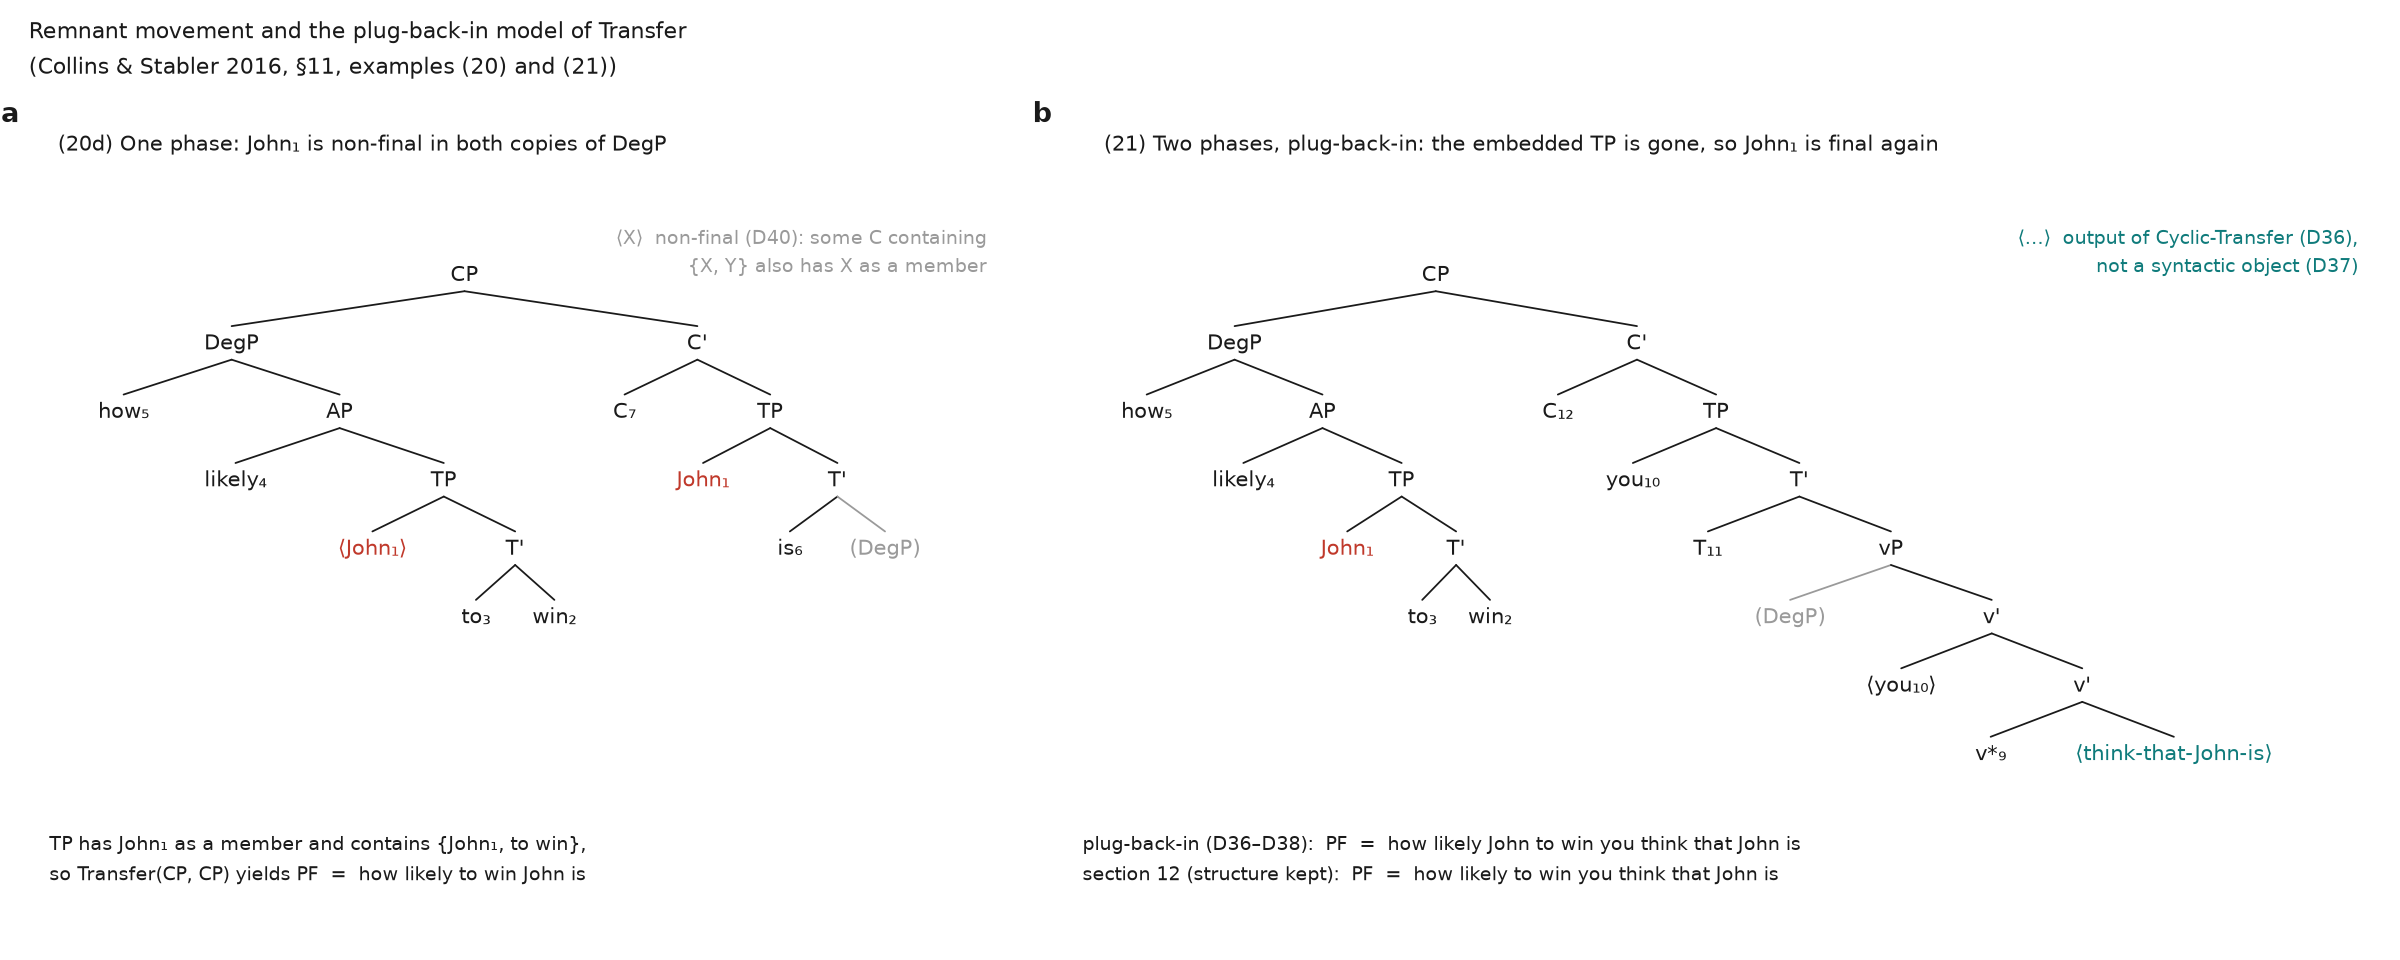
\includegraphics[width=\linewidth]{remnant_derivation.png}
  \caption{Remnant movement, C\&S (20) and (21), read off validated
  derivation objects: node labels from \Def{28}, daughter order from
  \Def{41}b, angle brackets (unpronounced) from \Def{40}. \textbf{(a)} In one
  phase, \pf{John}$_1$ is non-final in both copies of the DegP.
  \textbf{(b)} Across two phases under the plug-back-in model, the embedded
  TP has been replaced by a transferred pair, and \pf{John}$_1$ in the moved
  DegP is final.}
  \label{fig:remnant}
\end{figure}

Finally, \Thm{8} fails at every Cyclic-Transfer step under the plug-back-in
model: replacing a complement by a pair alters an object already built. C\&S
note this as one reason to reject the model; the implementation detects it
automatically on every derivation with a Cyclic-Transfer step.

% ================================================================ 6
\section{The Section 12 alternative}
\label{sec:ntc}

Section~12 of C\&S sketches an NTC-respecting Transfer: Transfer leaves the tree
unchanged and extends two functions, PF and LF; the transferred objects
are their domain; and ``the accessible parts of workspace $W$ are given by $W$
minus those already transferred''. The formal version was to appear in an
appendix that was not published. We implemented the sketch as
\code{NTCDerivation}, and it behaves as C\&S describe. \Thm{8} holds at
every Transfer step. No transferred pair enters the workspace, so \Def{7}
suffices and \Def{37} is not needed. The PIC still holds, though now as a
consequence of the accessibility condition. Example (21) is pronounced
\pf{how likely to win you think that John is}. On every derivation in which nothing moves out of a moved phrase, both models
yield the same PF and LF (Table~\ref{tab:regimes}). The sketch is
nevertheless under-determined in two respects.

\paragraph{What ``$W$ minus those already transferred'' removes.}
Read \emph{per occurrence}, an occurrence is inaccessible iff its path passes
through a transferred object. Read \emph{per object}, an object is
inaccessible iff it is contained in a transferred object. The two readings
come apart whenever something has moved to a phase edge: the edge copy is
accessible, but the same object also occurs inside the transferred
complement.

\begin{observation}
\label{obs:object}
Under the per-object reading, every derivation in which a phrase moves on
from a phase edge is underivable. This includes successive-cyclic
wh-movement, the embedded question, long subject wh-movement, and (21)
itself, the example Section~12 was introduced to rescue
(Table~\ref{tab:regimes}).
\end{observation}

\begin{table}[t]
\centering
\footnotesize
\begin{tabular}{@{}llll@{}}
\toprule
Derivation & Plug-back-in & \S12, occurrence & \S12, object \\
\midrule
\code{remnant_movement}      & \pf{how likely to win John is} & same & same \\
\code{remnant_across_phases} & \pf{how likely John to win you\dots} & \pf{how likely to win you\dots} & underivable \\
\code{successive_cyclic_wh}  & \pf{who you think John will see} & same & underivable \\
\code{you_wonder_who_john_will_see} & \pf{you wonder who John will see} & same & underivable \\
\code{who_does_sue_think_fell} & \pf{who Sue think fell} & same & underivable \\
\bottomrule
\end{tabular}
\caption{PF under the three Transfer regimes, for the derivations where they
differ or where the difference was expected. The other eight derivations with
a Transfer step give identical results under all three.}
\label{tab:regimes}
\end{table}

\paragraph{What a stage is.}
\Def{10} makes a stage a pair $\pair{\LA,W}$. Section~12 moves Transfer's
effect into PF and LF, which the stage does not contain. A Section~12
Transfer step therefore repeats the previous stage, which no clause of
\Def{38} licenses, and \Def{42}--\Def{44}, which require
$W_n=\{\pair{\mathrm{PHON},\mathrm{SEM}}\}$, do not apply. The repair is to
restate the stage as $\pair{\LA,W,\mathrm{PF},\mathrm{LF}}$, which is what
\code{NTCStage} does. Section~12 therefore changes the definition of a
derivation as well as the definition of Transfer.

% ================================================================ 7
\section{Theorem 4: tokens and chains}
\label{sec:t4}

We enumerated both $[T(\mathrm{Lex})]$ and $C(\mathrm{Lex})$ for the lexicon
$\{\mathit{John},\mathit{see}\}$ up to five Merge nodes, and mapped each
token class to the Chain-based object with the same structure and the image
of the same path (Table~\ref{tab:t4}).

\begin{table}[t]
\centering
\small
\begin{tabular}{@{}lrrrrrc@{}}
\toprule
\Def{14}$'$(c) & Size $\le$ & $|[T(\mathrm{Lex})]|$ & $|C(\mathrm{Lex})|$ & No image & $>1$ image & Bijection \\
\midrule
our reading & 1 &   3 &    3 &   0 &   0 & yes \\
our reading & 2 &   7 &    7 &   0 &   0 & yes \\
our reading & 3 &  25 &   23 &   2 &   0 & no \\
our reading & 4 & 123 &   95 &  28 &   0 & no \\
our reading & 5 & 703 &  437 & 272 &   6 & no \\
\midrule
dropped     & 1 &   3 &    3 &   0 &   0 & yes \\
dropped     & 2 &   7 &    7 &   0 &   0 & yes \\
dropped     & 3 &  25 &   27 &   0 &   2 & no \\
dropped     & 4 & 123 &  155 &   0 &  24 & no \\
dropped     & 5 & 703 & 1097 &   0 & 224 & no \\
\bottomrule
\end{tabular}
\caption{Token classes against Chain-based objects, by maximal number of
Merge nodes. In every row, every Chain-based object has a token preimage; the
failures are token classes with no image or with several.}
\label{tab:t4}
\end{table}

\paragraph{With the locality condition.}
The token system can move a lower token across a higher token of the same
lexical item, as in $\{\mathit{see}_2,\{\mathit{see}_3,\{\mathit{John}_1,
\mathit{see}_2\}\}\}$, which the driver derives. In the Chain-based system
the two \pf{see}s are the same object, and (c) forces the higher one to be
chosen, so the token class has no image. Remnant configurations fail in the
other direction: when an item sits inside both copies of a moved phrase,
neither occurrence c-commands the other, (c) admits both paths, and one token
class receives two Chain-based objects.

\paragraph{Without the locality condition.}
The Chain-based system records \emph{which} occurrence of an already-moved
item is re-merged; the token system does not (C\&S note that in the token
system ``the question \dots\ never arises''). One token class then has several
images.

\begin{observation}
Under each reading of \Def{14}$'$(c) we could construct, the natural
correspondence between $[T(\mathrm{Lex})]$ and $C(\mathrm{Lex})$ is a
bijection up to two Merge nodes and fails from three on.
\end{observation}

\noindent
We cannot rule out that the unpublished proof uses a different
correspondence. Any such correspondence would have to disregard the paths,
which are the information the Chain-based encoding adds.

% ================================================================ 8
\section{Selection and unordered triggers}
\label{sec:selection}

Triggered Merge (\Def{27}) licenses $\Merge(A,B)$ whenever $\Triggers(A)$ is
non-empty and $\Triggers(B)$ is empty; it never asks whether the trigger
feature \emph{matches} $B$. We enumerated every complete derivation from the
lexical array
\[\{\mathit{see}_1,\mathit{Chris}_2,\mathit{v}^*_3,
\mathit{John}_4,\mathit{T}_5,\mathit{Comp}_6\}\]
under \Def{27} and under
selectional variants (Table~\ref{tab:merge}).

\begin{table}[t]
\centering
\small
\begin{tabular}{@{}lrrrrc@{}}
\toprule
Merge rule & Derivations & Objects & Stages & PF strings & \Thm{5}, \Thm{6}, \Thm{8}, \Thm{9} \\
\midrule
\Def{27} Triggered Merge                & 6{,}267{,}280 & 648 & 4{,}072 & 6 & hold \\
+ selection, ranked triggers            &    55{,}968 &  12 &   280 & 6 & hold \\
+ selection, ranked, EPP needs D        &    27{,}984 &   6 &   178 & 4 & hold \\
+ selection, unranked triggers          &   171{,}424 &  24 &   448 & 6 & hold \\
+ selection, unranked, EPP needs D      &    85{,}712 &  12 &   304 & 4 & hold \\
\bottomrule
\end{tabular}
\caption{All complete derivations (\Def{15}) from one six-token lexical
array, under five Merge rules. \emph{Objects} counts distinct derived
objects; \emph{stages} counts distinct reachable stages.}
\label{tab:merge}
\end{table}

\Thm{5}, \Thm{6}, \Thm{8} and \Thm{9} hold on every reachable stage under
all five rules. They follow from the format of stages and workspaces
(\Def{10}, \Def{14}) and do not depend on the condition that licenses a
Merge.

Under plain \Def{27}, it makes no difference which trigger feature \Def{26}
checks, because only the number of remaining triggers matters. The ranked
and unranked policies give identical derivations, and a test confirms this.

Once selection is added, the choice does matter, and C\&S assume the
unranked case. Unranked selection doubles the number of derived objects (24
against 12). In each of the 12 extra objects, a head's EPP feature took a DP
as its complement and its selection feature was then satisfied by a
specifier. Four contain $[_{\mathrm{TP}}\ \mathrm{vP}\ [_{\mathrm{T'}}\
\mathrm{T}\ \mathrm{DP}]]$, C\&S's own example; eight show the same pattern
one phase down, $[_{\mathrm{vP}}\ \mathrm{VP}\ [_{\mathrm{v'}}\
\mathrm{v}^*\ \mathrm{DP}]]$. C\&S suggest that the NTC would block such
orders. That argument applies to a DP that moves into the complement
position; a DP merged there externally is not blocked by anything.

% ================================================================ 9
\section{Discussion}
\label{sec:discussion}

\paragraph{Agree and head movement.}
There is no Agree in the axiomatization: \Def{1} lists it, but C\&S do not
formalize it. Since $\TLF$ keeps the whole Sem set of every token, the only
way to obtain a derivation that crashes at CI is a lexical item that is
uninterpretable by stipulation. There is no head movement either, so
\pf{John Mary give flowers} and \pf{Mary not praise John}
(Figure~\ref{fig:neg}) come out in specifier--head--complement order without
an auxiliary. Both follow from the axioms as stated, and the implementation
leaves them as they are.

\paragraph{Extensibility.}
Adding a category the axioms do not mention costs only lexical entries.
Negation (Figure~\ref{fig:neg}) needs three lexical items and one selection
feature and no change to any definition; \Def{35} correctly treats NegP as
transparent. The embedded question (Figure~\ref{fig:wonder}) requires nothing
beyond an additional Comp. The one place where the category inventory is
hard-coded is \Def{35}, which enumerates the phase heads.

\begin{figure}[t]
  \centering
  \begin{minipage}[b]{0.44\linewidth}
    \centering
    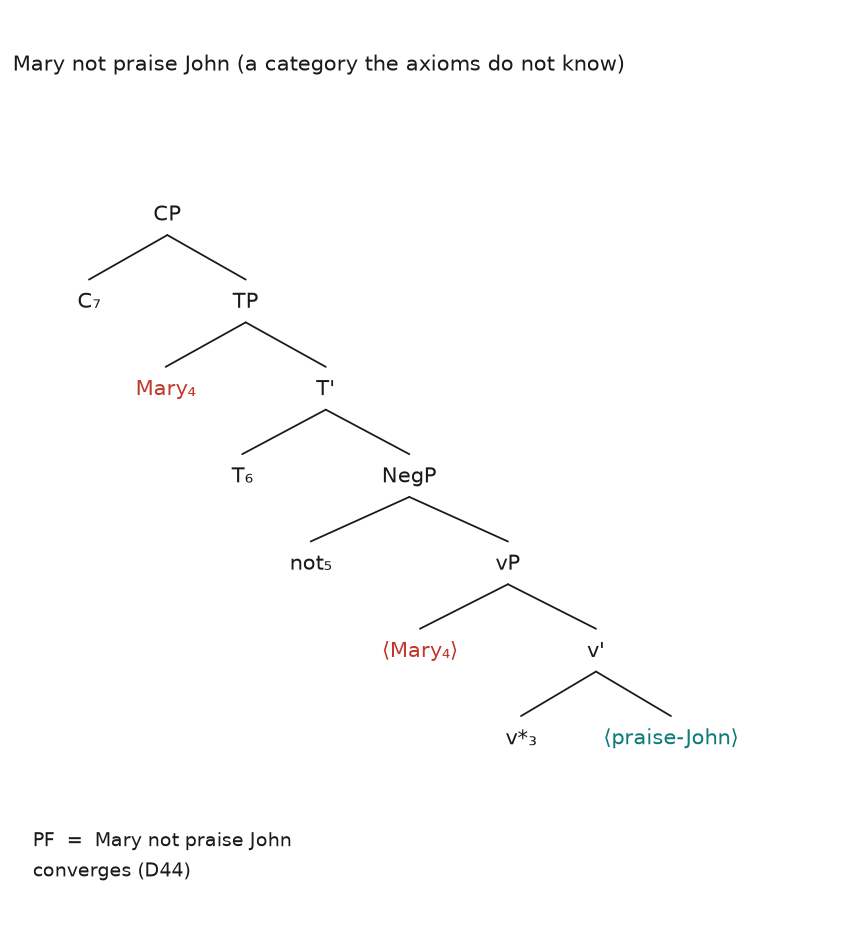
\includegraphics[width=\linewidth]{mary_not_praise_john.png}
    \caption{\pf{Mary not praise John}. Neg is added with no change to the
    definitions; the chunk transferred at the v* phase is identical to the
    affirmative one.}
    \label{fig:neg}
  \end{minipage}\hfill
  \begin{minipage}[b]{0.52\linewidth}
    \centering
    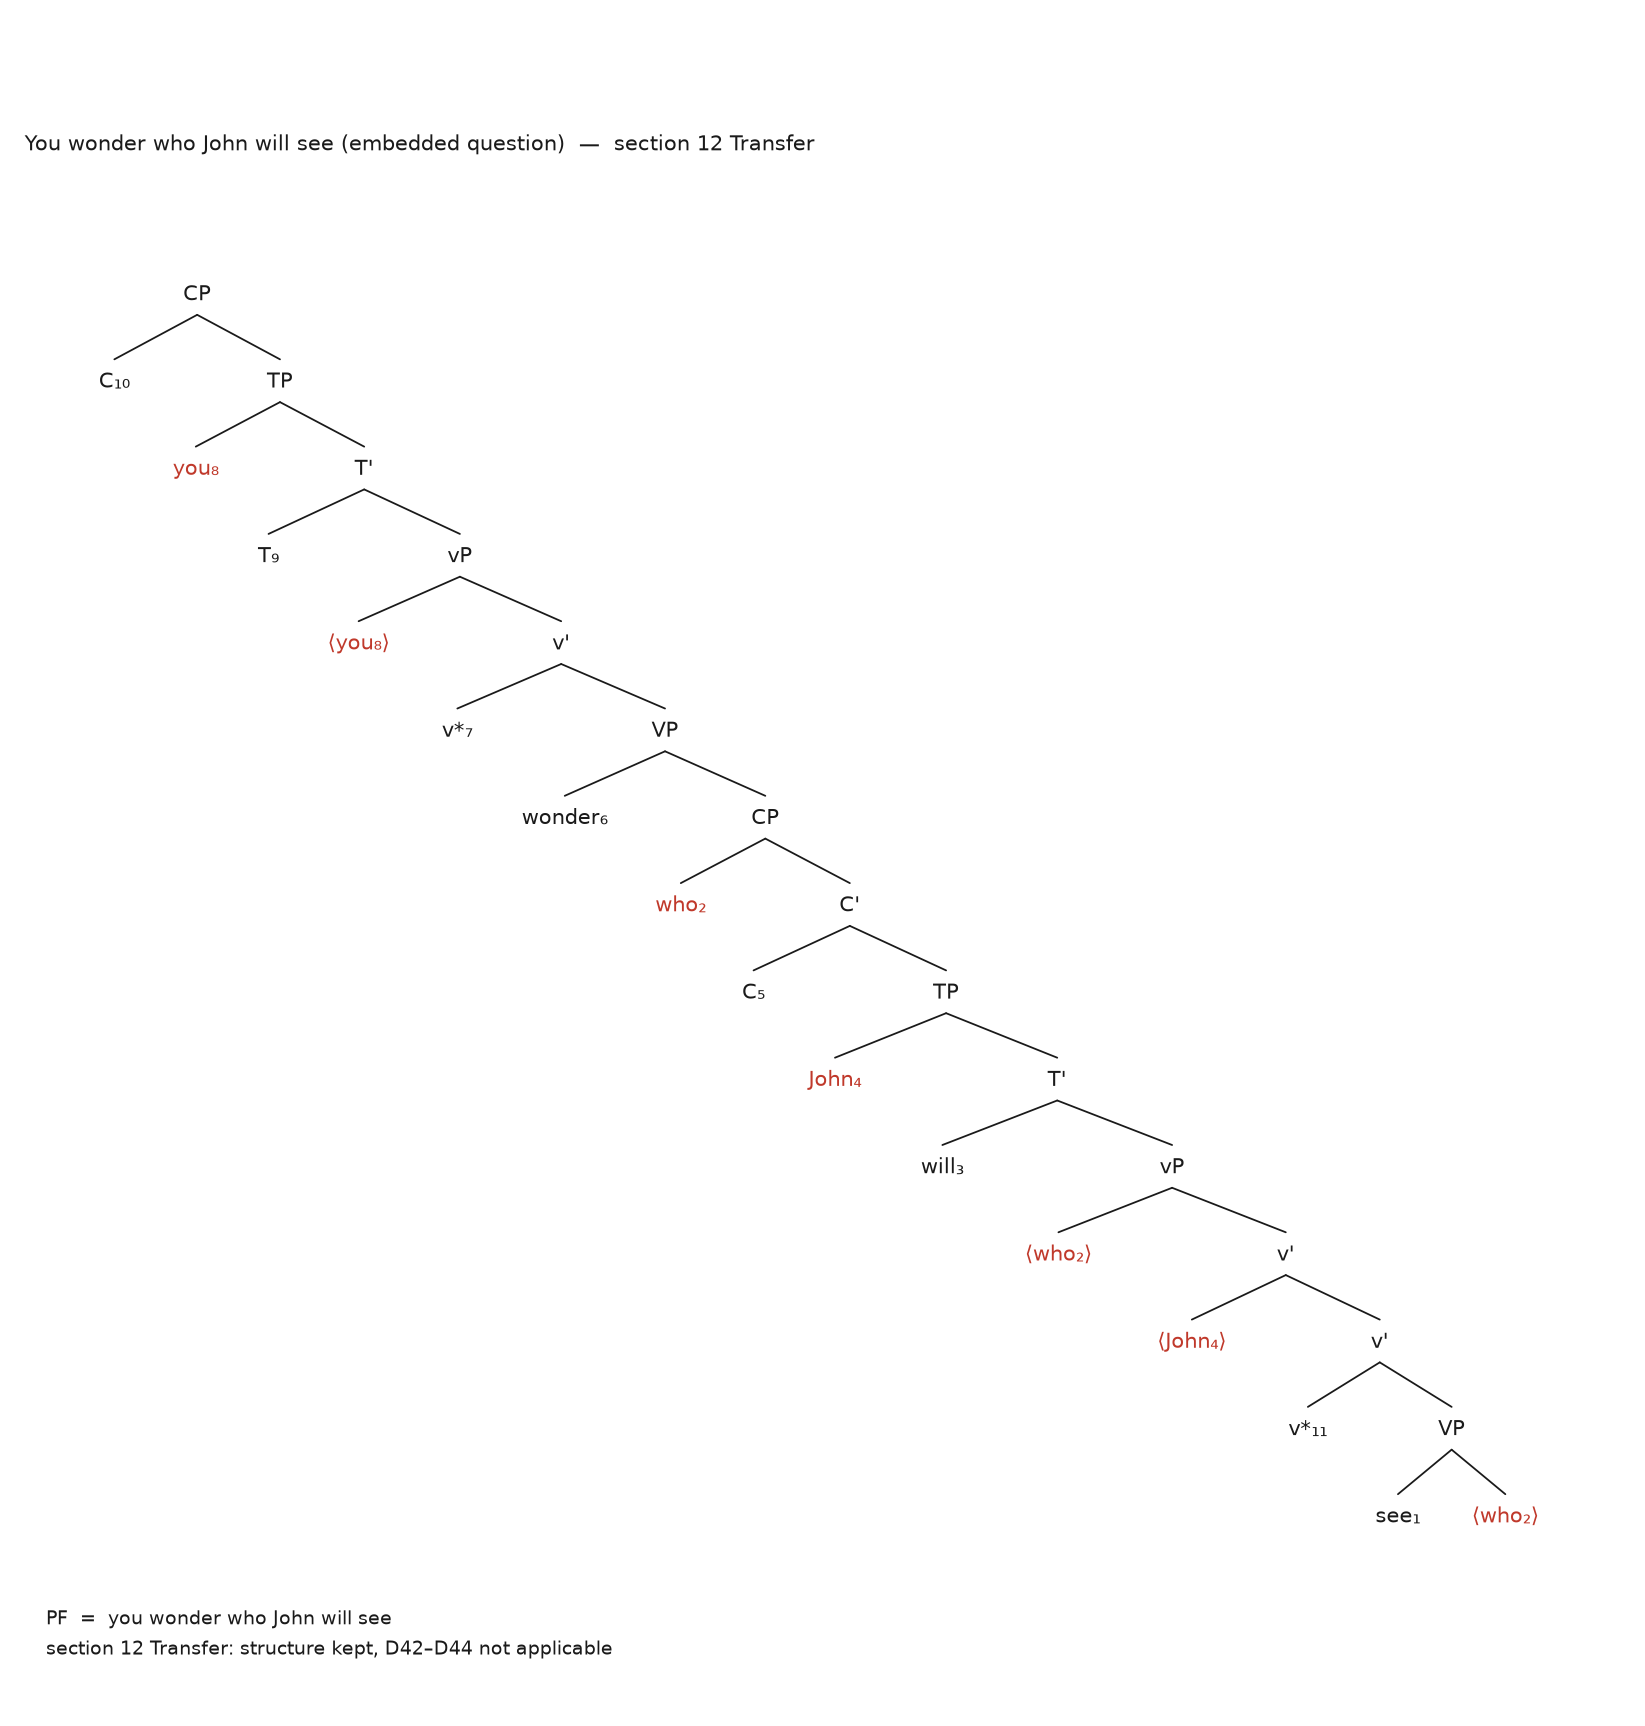
\includegraphics[width=\linewidth]{you_wonder_who_john_will_see.png}
    \caption{\pf{You wonder who John will see}. \pf{who}$_2$ moves through
    the embedded v* edge to the embedded Spec,CP, its only final occurrence
    (\Def{40}).}
    \label{fig:wonder}
  \end{minipage}
\end{figure}

\paragraph{Limitations.}
The exhaustive checks are bounded: Theorem~4 is checked up to five Merge
nodes over a two-word lexicon, and the Merge-rule comparison covers one
six-token array. A failure on a bounded fragment refutes the theorem as
stated, but a pass does not prove a general theorem. The PF column of
Table~\ref{tab:coverage} reflects the absence of morphology and head
movement in the axioms. It does not indicate errors in the implementation.

% ================================================================ 10
\section{Related work}
\label{sec:related}

Minimalist Grammars \citep{Stabler1997,Stabler2011} formalize feature-driven
Merge and Move as a grammar formalism with known generative capacity. C\&S formalize the
theory in the terms syntacticians use, and our implementation keeps those
terms. The token-based treatment of copies
continues \citet{Collins1997,Collins2002} and \citet{Gartner2002}; the
Chain-based alternative relates to \citet{Kracht2001} and to the treatment
of chains in \citet{Nunes2004}. Phases and the PIC follow
\citet{Chomsky2000,Chomsky2004}, and the plug-back-in model corresponds to
the ``conservative'' reading of Multiple Spell-Out in \citet{Uriagereka1999}.
The linearization in \Def{41} is LCA-based \citep{Kayne1994}. Approaches in
which every phrase is a phase \citep{Muller2010} or in which spell-out is
formulated differently \citep{EpsteinSeely2006} could be compared within the
same driver by replacing \Def{35} or \Def{36}.

% ================================================================ 11
\section{Conclusion}
\label{sec:conclusion}

Implemented as written, the C\&S definitions derive all of the paper's
examples, and Theorems \Thm{5}--\Thm{10} hold on every reachable stage we
checked. The implementation reproduces the paper's argument against the
plug-back-in model and shows in addition that the mispronounced derivation
of (21) converges. The problems we found are in parts that C\&S present as
sketches or whose proofs were not published. The Section~12 alternative
works only under the per-occurrence reading of accessibility and needs a
stage that records PF and LF. The natural correspondence of Theorem~4 fails
from three Merge nodes on. The same driver can be used to test other
definitions of phases, Transfer or selection against these derivations.

% ---------------------------------------------------------------- data
\section*{Code and data availability}

The code and data are available at
\url{https://github.com/norbmor/minimalist-cs2016}. The implementation is
standard-library Python~3; only the figure script requires matplotlib. The
following commands reproduce every number and figure in this report:

\begin{lstlisting}[language=bash]
python test_cs2016.py      # 55 checks
python test_sentences.py   # 21 checks
python derivations.py > derivation_report.txt
python sentences.py   > sentence_report.txt
python tables.py           # the three CSV tables
python figures.py          # the four figures
\end{lstlisting}

\noindent
\code{tables.py} writes the data of Tables~\ref{tab:regimes},
\ref{tab:t4} and~\ref{tab:merge}; \code{figures.py} draws
Figures~\ref{fig:wh}--\ref{fig:wonder}.

\noindent
Trace files are byte-reproducible under any hash seed, and figures are drawn
from validated derivation objects, so a figure cannot show a structure the
axioms did not build.

% ---------------------------------------------------------------- refs
\bibliographystyle{plainnat}
\bibliography{references}

% ---------------------------------------------------------------- appendix
\appendix
\section{Changes from the 2011 manuscript}
\label{app:2011}

\begin{itemize}[leftmargin=*,itemsep=2pt]
\item Numbering changed throughout. For example, Triggers is \Def{27} in 2011
  and \Def{26} in 2016; Triggered Merge \Def{28}$\to$\Def{27}; Label
  \Def{29}$\to$\Def{28}; strong phase \Def{38}$\to$\Def{35}; TransferPF
  \Def{42}$\to$\Def{41}; PIC \Thm{13}$\to$\Thm{14}; NTC \Thm{7}$\to$\Thm{8}.
\item \Def{14} is now the definition of a derivation (2011's
  \Def{14}/\Def{22}/\Def{23} merged); an empty final lexical array and a
  single root are \Def{15}.
\item \Def{35} requires a strong phase to be a maximal projection, and
  \Def{38} bars Transfer while an embedded phase's complement is
  untransferred. The implementation checks both; all derivations satisfy
  them.
\item \Def{40} replaced the 2011 c-command definition of finality. This is
  why the 2011 variants of Cyclic-Transfer and TransferPF for lower copies
  (\Def{36}$'$, \Def{36}$''$, \Def{42}$'$, \Def{42}$''$) are gone, and why
  remnant movement within one phase now works with a single Cyclic-Transfer.
\item Section~5 (Chains, Theorem~4) is new in 2016.
\item The 2016 version states that trigger features are unordered. The
  implementation's ranking is kept only to name which feature is checked,
  and is inert under \Def{27} (Section~\ref{sec:selection}).
\end{itemize}

\end{document}
